\documentclass[12pt]{article}
\usepackage{amsmath}
\usepackage{graphicx}
\usepackage{hyperref}
\usepackage[latin1]{inputenc}

\title{Progetto di Programmazione}
\author{Nome : n. matricola}
\date{settembre 2023}

\begin{document}
\maketitle

\begin{figure}[h]
    \centering
    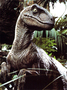
\includegraphics{raptor.jpg}
    % qui ci va il logo dell'unibo ma ora non me lo fa mettere
\end{figure}

\newpage


\section*{Suddivisione dei compiti}
\subsection*{Davide}
\begin{itemize}
    \item Menu principale
    \item Menu di pausa
\end{itemize}
File: Menu, Menu\_playing
 
\subsection*{Elia}
\begin{itemize}
    \item Nemici 
    \item Sistema di combattimento
\end{itemize}
File: Boom, Character, Chaser, Coward, Drunk, Enemy, Flyer, Projectile, Shooter, Stalker, Time, Turret

\subsection*{Matteo}
\begin{itemize}
    \item Artefatti
    \item Hero
    \item Sistema di combattimento
\end{itemize}
File: Artifact, Hero

\subsection*{Mattia}
\begin{itemize}
    \item Creazione e gestione delle stanze 
    \item Strutture dati per la loro memorizzazione
    \item Grafica
\end{itemize}
File: Board, Templates, GeneralTemplate, Room, Door, Wall

\newpage
\section*{Scelte implementative}
\subsection*{Il Gioco}
La classe Menu gestisce il menù principale, mentre la classe Game si occupa di gestire tutto ciò che riguarda il gioco.
% brutto come è scritto
Game comprende 3 finestre (per la grafica delle stanze, delle staistiche del personaggio e per il punteggio), il personaggio (Hero), l'indice delle stanze e un puntatore alla stanza corrente.

\subsection*{Le Stanze}
Ogni stanza contiene un puntatore alle stanze con cui confina che sono già state esplorate, in modo da potersi muovere in una di queste senza visitare l'indice; delle coordinate x e y per identificarla univocamente all'interno della mappa, dei flag per gestire lo stato di ogni porta (aperta/chiusa presente/non presente), e un template. Il template contiene i muri, le porte, i nemici e gli artefatti.
Le stanze sono memorizzate in una struttura dati di tipo vettore, chiamata indice, in modo da potere essere aggiunte gradualmente esplorando la mappa; l'indice viene usato solo quando si crea una nuova stanza per avere delle porte coerenti con il resto della mappa.
In questo modo il cambio di stanza quando si torna in una stanza già visitata è molto rapido, mentre è necessariamente più lento quando se ne visita una nuova. 

\subsection*{I Template}
Per il contenuto delle stanze si usa una classe che memorizza il contenuto della stanza, detta template, ce ne sono 39, di diverse rarità e ogni volta che si crea una nuova stanza, gliene ne viene asseganto uno.
Per potere essere interscambiabili i template sono tutti sottoclassi di GeneralTemplate e sono memorizzati all'interno della stanza come puntatori.
I muri, le porte, i nemici e gli artefatti sono tutti memorizzati in array dinamici in modo da potere variare in numero e contenuto per ogni stanza, anche tra quelle con lo stesso template.
Il file GeneralTemplate.cpp contiene delle funzioni per aggiungere alle stanze, insiemi di muri o porte in modo che abbiano una certa forma.

\subsection*{Il Personaggio}
La classe Hero controlla tutte le caratteristiche dell'Eroe: vita, danno, chiave (per aprire porte), reload, range e abilità.
Le caratteristiche dell'eroe prendono valori diversi a seconda della classe che viene scelta prima di iniziare a giocare. Diverse classi possono avere quindi più o meno vita, range, danno e così via.
La funzione "useAbility" attiva abilità differenti a seconda della classe selezionata.
Le abilità possono modificare temporaneamente le caratteristiche dell'eroe o ripristinargli la vita.
La funziona "attack" crea un nuovo proiettile nella direzione voluta. "CenterHero" serve a posizionare il personaggio al centro della stanza quando inizia il gioco. 
Tutte le restanti funzioni modificano le variabili del personaggio. Per esempio "useKey" consuma la chiave del personaggio e apre una porta, "increaseHealth" aumenta la vita.


\subsection*{I Nemici}

\subsection*{Gli artefatti}
Gli Artefatti sono creati come semplici Drawable. Sono quindi dei caratteri presenti nelle stanze di gioco, con cui possiamo interagire. Essi vengono creati insieme al Template della stanza. A differenza dei nemici che vengono creati casualmente, essi vengono posizionati in punti precisi. Questo per non permettere la generazione in luoghi troppo facili da raggiungere.
Esistono tre tipi di artefatti: Range, Danno e Vita.
Possono rendere il gioco più facile con l'aumentare dello score, ma è bilanciato dall'aumento progressivo della difficoltà.

\subsection*{Il sistema di combattimento}
Il sistema di combattimento regola danno inflitto e danno subito da nemici ed eroe. 
...

\end{document}












